%%% Preamble
\documentclass[paper=a4, fontsize=11pt]{scrartcl}
\usepackage[T1]{fontenc}
\usepackage{fourier}
\usepackage[brazilian]{babel}							% Português
\usepackage[protrusion=true,expansion=true]{microtype}	
\usepackage{amsmath,amsfonts,amsthm} % Math packages
\usepackage[pdftex]{graphicx}
\usepackage{graphicx}	
\usepackage{url}
\usepackage{indentfirst}
\usepackage{mathtools}
\usepackage{listings}
\usepackage[titletoc]{appendix}
\usepackage{float}
\usepackage{courier}
\usepackage[export]{adjustbox}
\DeclarePairedDelimiter{\Vector}{\lparen}{\rparen}

%%% Custom sectioning
\usepackage{sectsty}
\allsectionsfont{\centering \normalfont\scshape}


%%% Custom headers/footers (fancyhdr package)
\usepackage{fancyhdr}
\pagestyle{fancyplain}
\fancyhead{}											% No page header
\fancyfoot[L]{}											% Empty 
\fancyfoot[C]{}											% Empty
\fancyfoot[R]{\thepage}									% Pagenumbering
\renewcommand{\headrulewidth}{0pt}						% Remove header underlines
\renewcommand{\footrulewidth}{0pt}						% Remove footer underlines
\setlength{\headheight}{13.6pt}

%%% Maketitle metadata
\newcommand{\horrule}[1]{\rule{\linewidth}{#1}} 		% Horizontal rule

\title{
		%\vspace{-1in} 	
		\usefont{OT1}{bch}{b}{n}
		\normalfont \normalsize \textsc{Insper: Instituto de Ensino e Pesquisa} \\ [25pt] %Instituição
		\horrule{0.5pt} \\[0.4cm]														  
		\huge Implementação e análise de treliças planas \\			%Título do relatório
		\horrule{2pt} \\[0.5cm]
}
\author{										%Autores
		\normalfont 								\normalsize
        Marcelo Andrade\\[-3pt]		\normalsize
		Pedro Cunial\\[-3pt]		\normalsize
        Gabriela Almeida\\[-3pt]		\normalsize
}
\date{\today}

%%% Confs codigo
\lstset{basicstyle=\footnotesize\ttfamily}


%%% Início document
\begin{document}
	
%%% Capa do documento
\maketitle

\newpage

%% Sumário
\tableofcontents

\newpage

%%% Início Relatorio

%%% Objetivos
\section{Objetivos} \label{sec:objetivos}
Os objetivos do projeto são os seguintes:

\begin{itemize}
	\item Implementar um programa para análise de tração/compressão em
	treliças planas. O código deverá ser escrito de modo que os dados de entrada
	possam ser facilmente alterados a partir de um arquivo de texto. O programa deverá gerar um arquivo de saída.
	
	\item Aplicar técnicas numéricas e implementar um programa para
	solução de sistemas de equações. 
	
	\item Analisar o arquivo de saída com o pós-processamento dos dados
	disponibilizado. 
\end{itemize}

%%% Introdução
\section{Introdução}

Com base nos conceitos desenvolvidos na disciplina de Transferência de Calor e Mecânica dos Sólidos sobre treliças plana, dever-se-ia desenvolver um projeto que cumpriria os objetivos listados na seção \ref{sec:objetivos}

Na primeira parte do projeto, era preciso usar os modelos fornecidos de entrada e saída e implementar uma função capaz de executar os procedimentos discutidos em aula, para enfim, analisar a o valor de tração/compressão em treliças planas. Para desenvolver essa etapa do projeto, decidiu-se utilizar a linguagem Python para resolver os sistemas de equações.

Em uma segunda parte, era necessário usar técnicas numéricas discutidas em aula, implementando um solucionador de sistemas de equações para resolver o sistema obtido na parte I do projeto. As técnicas numéricas discutidas em aula foram a de Gauss-Seidel e a de Jacobi. Após implementar ambas as técnicas e comparar os resultados obtidos por cada uma delas, decidiu-se usar a Gauss-Seidel, pois ela apresentou os valores de saída mais condizentes com o projeto.

%%% Metodologia
\section{Metodologia}

A partir do arquivo de entrada do programa, primeiramente calcula-se os graus de liberdade de cada um dos elementos a partir da matriz de incidências do arquivo de entrada. Sendo \(N\) os graus de liberdade de um elemento \(x\), e \(I\) a matriz de incidências:


\[N_x = 
\begin{bmatrix}
I_{x1} - 1 ,& I_{x1} ,& I_{x2} - 1 ,& I_{x2}  \\
\end{bmatrix}
\]

Em seguida, calcula-se as especificações de cada elemento da treliça a partir da matriz de coordenadas \(C\), sendo elas o comprimento do elemento, cosseno e seno do ângulo. Considerando \(L\) o comprimento do elemento \(x\), \(cos\) o cosseno do ângulo \(\theta\) de \(x\) e \(sin\) o seno do ângulo \(\theta\) de \(x\):

\[L_x = \sqrt{(x_2 - x_1)^2 + (y_2 - y_1)^2}\]

\[sin_x = \frac{y_2 - y_1}{L_x}\]

\[cos_x = \frac{x_2 - x_1}{L_x} \]

Com as especificações de cada elemento obtidas, calcula-se as matriz de rigidez do elemento de barra no sistema global, representada por \(K_e\). Sendo \(E\) o módulo de elasticidade do material da barra, \(A\) a área da seção transversal da barra, \(l\) o comprimento da mesma e \(c\) e \(s\) respectivamente o cosseno e seno do ângulo \(\theta\) do elemento:

\[K_e = \frac{E \cdot A}{l}
\begin{bmatrix}
c^2 & cs & -c^2 & -cs\\
cs & s^2 & -cs & -s^2 \\
-c^2 & -cs & c^2 & cs \\
-cs & -s^2 & cs & s^2
\end{bmatrix}
\]

Já com a matriz de rigidez no sistema global de cada elemento, calculou-se a matriz de rigidez global da treliça, representada por \(K_g\). Para esse cálculo, primeiro tem-se que determinar as matrizes de superposição para cada elemento, a soma dessas matrizes resulta na rigidez global da treliça. 
	
As matrizes de superposição são obtidas através substituição dos índices da matriz \(K_e\) pelos seus respectivos graus de liberdade.

A partir da matriz \(K_g\), utilizando o vetor de forças globais e os graus de liberdade dos nós, aplica-se as condições de contorno na matriz \(K_g\).

Com a matriz \(K_g\) simplificada para a análise e a usando a matriz de forças \(P_g\), foi-se calculado o vetor de deslocamento dos nós da treliça, representada por \(U\).

\[[K_g]\cdot\{U\} = \{P_g\}\]

Pode-se interpretar a equação matricial acima como um sistema de equações. Utilizou-se o método numérico de Gauss-Seidel, como é explicado em \cite{gauss_seidel}. Usamos como entrada do método um número máximo de 1000 iterações e um erro esperado igual a 0 com precisão de ponto flutuante, resultando nos valores do vetor de deslocamento.

Com o vetor de deslocamento calculado e utilizando a matriz \(K_g\) anterior as condições de contorno descritas, aplicamos condições de contorno no vetor \(U\) e na matriz \(K_g\) e determinou-se as reações de apoio em cada um dos nós da treliça, formando uma matriz \(R\) de reações.

\[\{R\} = [K_g] \{U\}\]

Por fim, calculou-se a tensão e deformação de cada um dos elementos, a tensão representado por \(\sigma\) e a deformação representada por \(\epsilon\).

\[\sigma = \frac{E}{l}  
\begin{bmatrix}
-c & -s & c & s\\
\end{bmatrix}
\begin{bmatrix}
u_1 \\
v_1 \\
u_2 \\
v_2 \\
\end{bmatrix}
\]


\[\epsilon = \frac{1}{l}  
\begin{bmatrix}
-c & -s & c & s\\
\end{bmatrix}
\begin{bmatrix}
u_1 \\
v_1 \\
u_2 \\
v_2 \\
\end{bmatrix}
\]

Com todos os valores das reações de apoio, tensões e deformações dos elementos, e deslocamentos dos nós, formatou-se-os em um arquivo de saída, como pode ser visto no apêndice \ref{appendix:saida}. 

%%% Resultados e Discussão
\section{Resultados e Discussão}

A partir da treliça de entrada representada pela figura \ref{fig:trelica_entrada}, construiu-se o arquivo de entrada do programa, como visto do apêndice \ref{appendix:entrada}.

\begin{figure}[H]
	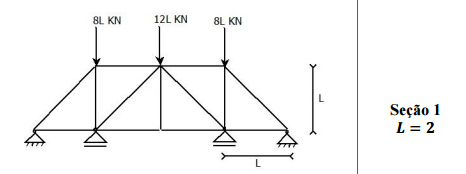
\includegraphics[width=\textwidth]{trelica_entrada.png}
	\caption{Representação da treliça de entrada do programa}
	\label{fig:trelica_entrada}
\end{figure}

\begin{figure}[H]
	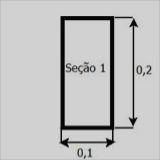
\includegraphics[center]{secao1.png}
	\caption{Representação da seção transversal da treliça de entrada}
	\label{fig:secao14}
\end{figure}


Para validar os resultados obtidos, montou-se a mesma treliça do arquivo de entrada no programa Ftool com intuito de se comparar os valores das reações de apoio.

\begin{figure}[H]
	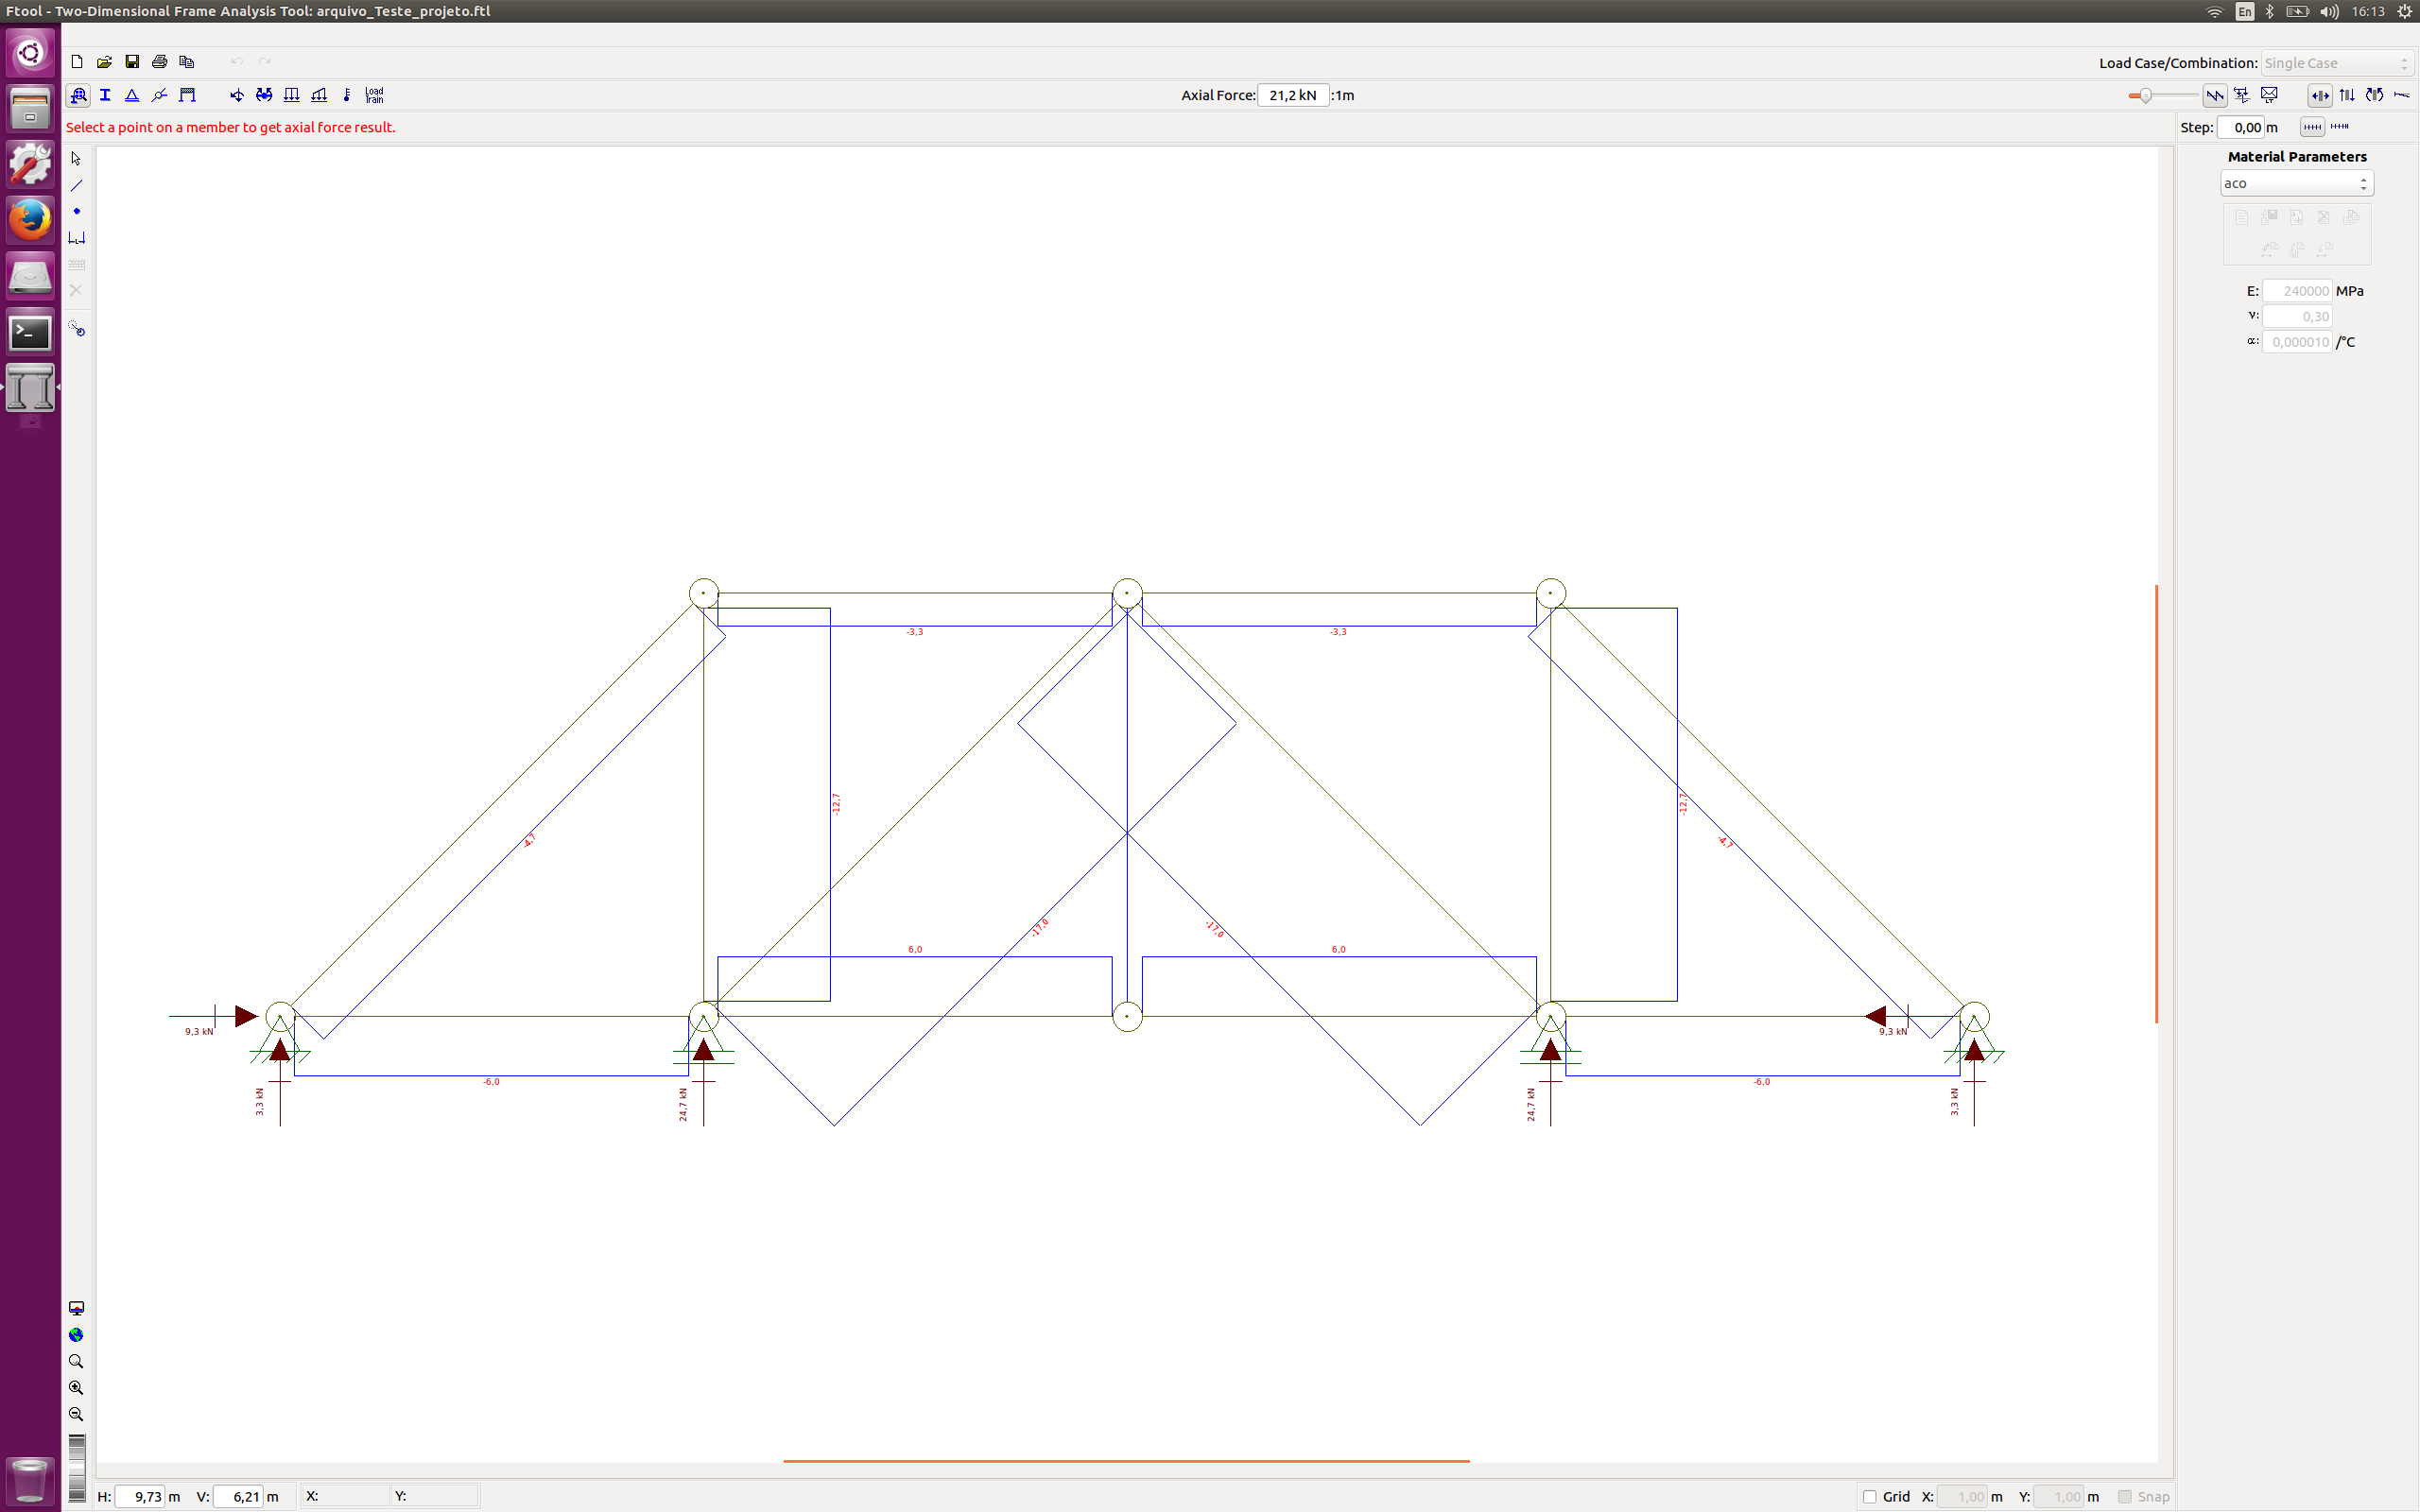
\includegraphics[width=\textwidth]{ftool.png}
	\caption{Implementação da entrada do programa no Ftool}
	\label{fig:ftool}
\end{figure}

Como pode ser observado na figura \ref{fig:ftool}, os valores encontrados a partir do Ftool condizem com os valores computados pelo programa feito pelo grupo. Há uma pequena diferença entre os resultados, que pode ser principalmente associada à utilização do método numérico de Gauss-Seidel para a resolução dos sistemas lineares. O método usado pelo Ftool não é o mesmo usado pelo programa, causando uma diferença no resultado final.

%%% Conclusões
\section{Conclusões}

Softwares de simulação física são muito comuns nos dias de hoje. Após o projeto, podemos concluir que a elaboração de um software do mesmo tipo, ainda que menos profissional do que os utilizados pela indústria, pode não só ser uma tarefa consideravelmente simples, mas também uma ótima oportunidade de aprendizado.

Além disso, o conhecimento de métodos numéricos para manipulação de dados é extremamente importante na formação de um engenheiro (principalmente de computação), pois além de agregar um conhecimento técnico de como utilizá-los, sua compreensão permite entender as limitações da computação numérica atualmente, adicionando um enorme conhecimento ao ferramental de um desenvolvedor em termos não só de performance como também de escalabilidade de projetos.

\bibliography{referencias}{}
\bibliographystyle{plain}

\begin{appendices}
	\section{Arquivo Saída} \label{appendix:saida}
	
		\begin{lstlisting}
	*DISPLACEMENTS
		1 0.0 0.0
		2 1.577956428087981e-06 -6.041091190959638e-06
		3 -2.8571428571428564e-06 0.0
		4 2.3997541478958825e-22 -1.9019583569978225e-05
		5 0.0 -1.9019583569978225e-05
		6 -1.5779564280879803e-06 -6.041091190959638e-06
		7 2.8571428571428564e-06 0.0
		8 0.0 0.0
	
	*ELEMENT_STRAINS
		1 -1.1157836907179139e-06
		2 -1.4285714285714282e-06
		3 -3.020545595479819e-06
		4 -7.889782140439904e-07
		5 1.4285714285714282e-06
		6 0.0
		7 -4.040610178208841e-06
		8 -7.889782140439903e-07
		9 1.4285714285714282e-06
		10 -4.040610178208841e-06
		11 -3.020545595479819e-06
		12 -1.115783690717914e-06
		13 -1.4285714285714282e-06
	
	*ELEMENT_STRESSES
		1 -234314.57505076192
		2 -299999.99999999994
		3 -634314.5750507619
		4 -165685.424949238
		5 299999.99999999994
		6 0.0
		7 -848528.1374238566
		8 -165685.42494923796
		9 299999.99999999994
		10 -848528.1374238566
		11 -634314.5750507619
		12 -234314.57505076195
		13 -299999.99999999994
	
	*REACTION_FORCES
		1 FX = 9313.708498984757
		1 FY = 3313.708498984759
		3 FY = 24686.291501015236
		7 FY = 24686.291501015236
		8 FX = -9313.708498984757
		8 FY = 3313.70849898476
	\end{lstlisting} 
	
		\section{Arquivo Entrada} \label{appendix:entrada}
		
		\begin{lstlisting}
	*COORDINATES
	8
	1 0 0
	2 2 2
	3 2 0
	4 4 2
	5 4 0
	6 6 2
	7 6 0
	8 8 0
	
	*ELEMENT_GROUPS
	13
	1 1 BAR
	2 1 BAR
	3 1 BAR
	4 1 BAR
	5 1 BAR
	6 1 BAR
	7 1 BAR
	8 1 BAR
	9 1 BAR
	10 1 BAR
	11 1 BAR
	12 1 BAR
	13 1 BAR
	
	*INCIDENCES
	1 1 2
	2 1 3
	3 2 3
	4 2 4
	5 3 5
	6 4 5
	7 3 4
	8 4 6
	9 5 7
	10 4 7
	11 6 7
	12 6 8
	13 7 8
	
	*MATERIALS
	13
	210E9 1570E6 1570E6
	210E9 1570E6 1570E6
	210E9 1570E6 1570E6
	210E9 1570E6 1570E6
	210E9 1570E6 1570E6
	210E9 1570E6 1570E6
	210E9 1570E6 1570E6
	210E9 1570E6 1570E6
	210E9 1570E6 1570E6
	210E9 1570E6 1570E6
	210E9 1570E6 1570E6
	210E9 1570E6 1570E6
	210E9 1570E6 1570E6
	
	*GEOMETRIC_PROPERTIES
	13
	2E-2
	2E-2
	2E-2
	2E-2
	2E-2
	2E-2
	2E-2
	2E-2
	2E-2
	2E-2
	2E-2
	2E-2
	2E-2
	
	*BCNODES
	6
	1 1
	1 2
	3 2
	7 2
	8 1
	8 2
	
	*LOADS
	3
	2 2 -16E3
	4 2 -24E3
	6 2 -16E3
		\end{lstlisting} 
\end{appendices}

%%% Fim do Documento
\end{document}